\documentclass[]{article}

%opening
\usepackage{graphbox}	% permette di modificare i margini
\usepackage{graphicx}
\usepackage{float}
\usepackage{longtable}
\usepackage{array}
\usepackage{fancyhdr}
\pagestyle{fancy}

\newcommand{\copertina}{
	\begin{titlepage}
		\begin{center}
			
			\vspace{1cm}
			
			\begin{Huge}
				\textbf{Centro Estetico Nirvana} \\
			\end{Huge}
			
			\vspace{9pt}  
			
			\begin{large}
				\textbf{Progetto per il corso di Tecnologie Web\\}
				\textbf{A.A.} 2022/2023\\
				\vspace{3pt}
			\end{large}	  
			
			\vspace{24pt}
			
			\begin{large}
				\textbf{Indirizzo sito web:} \emph{http://tecweb.studenti.math.unipd.it/nbaesso}\\
			\end{large} 
			
			\vspace{10pt} 
			
			\bgroup
			\def\arraystretch{1.3}
			\centering
			\begin{tabular}{r|L{5cm}}
			\multicolumn{2}{c}{\textbf{Informazioni sul gruppo} } \\ \hline
			\textbf{Membri} &  Nicola Baesso - 2011877 \newline Matteo Cusin - 2008073 \newline Annalisa Egidi - 1216745 \newline Lisien Skenderi - 2023461\\
			\end{tabular}
			\egroup
			
			\begin{center}
				\textbf{Referente\\}
				Nicola Baesso - nicola.baesso@studenti.unipd.it\\
				\textbf{Utenti (credenziali username-password):\\}
				\textit{Amministratore:} admin - admin\\
				\textit{Cliente:} user - user\\
			\end{center}
			
		\end{center}
	\end{titlepage}
}	%FINE NEW COMMAND COPERTINA

\usepackage{lastpage}
\usepackage{fancyhdr}
\fancypagestyle{plain}{
	% cancella tutti i campi di intestazione e piè di pagina
	\fancyhf{}
	
	\lhead{
		Centro Estetico Nirvana
	}
	
	\lfoot{ %piè di pagina a sx
		Relazione Progetto Tecnologie Web
	}
	\rfoot{Pagina \thepage{} di \pageref{LastPage}} %es: pag: 4 di 10
	
	%linea orizzontale alle posizioni top e bottom della pagina (se è 0, non c'è la linea)
	\renewcommand{\headrulewidth}{0.3pt}  
	\renewcommand{\footrulewidth}{0.3pt}
}
\pagestyle{plain}

%\usepackage{calc} %introduce la notazione infissa per le op. aritmetiche interne a LaTeX

\usepackage[utf8]{inputenc}
%\usepackage{cm-super}

\usepackage{lmodern}
\usepackage[T1]{fontenc}
\usepackage[italian]{babel} %il documento è in italiano
%\usepackage{textcomp} %The pack­age sup­ports the Text Com­pan­ion fonts, which pro­vide many text sym­bols
%(such as baht, bul­let, copy­right, mu­si­cal­note, onequar­ter, sec­tion, and yen), in the TS1 en­cod­ing.

\usepackage{graphicx}       %permette di inserire delle immagini
\usepackage{caption}        %numerazione figure e loro descrizione testuale
\usepackage{subcaption}     %sottofigure numerabili
\usepackage{float}  %permette di inserire un # qualsiasi di figure fluttuanti
\usepackage[dvipsnames,table]{xcolor}
\usepackage{rotating} %permette di ruotare le immagini
%\usepackage{changepage} %utile se c'è bisogno di aggiustare margini per centrare figure

\usepackage{listings} %permette di inserire degli spezzoni di codice

\usepackage{tikz} %disegno di immagini vettoriali a schermo. Utile per grafi
\usetikzlibrary{arrows.meta}
\usetikzlibrary{graphs}
\usetikzlibrary{arrows}
%\usepackage{tikz-uml} %serve per disgnare l'UML, fantastica guida:
%https://perso.ensta-paristech.fr/~kielbasi/tikzuml/var/files/doc/tikzumlmanual.pdf
%download package: http://perso.ensta-paristech.fr/~kielbasi/tikzuml/

%package per le tabelle
\usepackage{booktabs} %permette di poter usare delle liste nelle tabelle
\usepackage{tabularx} 
\usepackage{longtable} %una tabella può continuare su più pagine
\usepackage{multirow} %utile per visualizzare una cella su più righe
%\usepackage{multicolumn} %cella su più colonne
%\usepackage[table]{xcolor} %rende disponibile l'utilizzo di un colore per lo sfondo
%delle celle di una tabella

%crea una cella per le tabelle in grado di andare a capo con \newline
%https://tex.stackexchange.com/questions/12703/how-to-create-fixed-width-table-columns-with-text-raggedright-centered-raggedlef
\usepackage{array}
\newcolumntype{L}[1]{>{\raggedright\let\newline\\\arraybackslash\hspace{0pt}}m{#1}}
\newcolumntype{C}[1]{>{\centering\let\newline\\\arraybackslash\hspace{0pt}}m{#1}}
\newcolumntype{R}[1]{>{\raggedleft\let\newline\\\arraybackslash\hspace{0pt}}m{#1}}


%indice con i puntini
\usepackage{tocloft}
\renewcommand\cftsecleader{\cftdotfill{\cftdotsep}}

%http://ctan.mirror.garr.it/mirrors/CTAN/macros/latex/contrib/appendix/appendix.pdf
\usepackage{appendix} %aggiunge dei comandi per l'appendice
\usepackage{parskip} %aiuta LaTeX a trovare il miglior stile per i page break
\setcounter{secnumdepth}{5} % numera i sottoparagrafi
\setcounter{tocdepth}{5} %aggiunge all'indice i sottoparagrafi
%\usepackage{titlesec} %\begin{paragraph} si può usare come subsubsubsection!

\usepackage{breakurl}%\url{...} può continare alla linea successiva. (si può andare a capo)

\usepackage[colorlinks=true]{hyperref}
\hypersetup{
	colorlinks=true,
	citecolor=black,
	filecolor=black,
	linkcolor=black, % colore dei link interni
	urlcolor=Maroon  % colore dei link interniesterni
}

%per alcune liste, permette di usare 'alligator' nei labeling 
\usepackage{blindtext} 
\usepackage{scrextend} 
\addtokomafont{labelinglabel} 
{\sffamily}

%FILE INCLUSI
\usepackage{graphicx}

\begin{document}

\copertina
\tableofcontents
\newpage
\section{Introduzione}
Il centro estetico Nirvana vuole implementare un sito Internet al fine di poter fornire informazioni riguardo al centro stesso.\\
Il sito dovrà contenere informazioni riguardo i trattamenti disponibili e i macchinari utilizzati per essi, nonchè informazioni sulle consulenze e ogni informazione relativa a dove si trova il centro e quali orari di apertura osserva.\\
Inoltre, permette agli utenti di richiedere una consulenza o un trattamento, che necessita di essere confermato o meno dal centro stesso. Le prenotazioni possono anche inserite, oltre che confermate o smentite, anche dal centro stesso.\\
É fondamentale che il sito garantisca accessibilitá, in modo da permettere a chiunque di poter essere utilizzato, e usabilitá, separando struttura, presentazione e comportamento.\\
Si vuole infine garantire una navigazione fluida tra i contenuti del sito, evitando al piú possibile il disorientamento e prevedendo il giusto supporto per ritornare all'interno del sito stesso.\\
\section{Analisi}
\subsection{Studio dell'utenza finale}
Il sito vuole fornire informazioni riguardanti i possibili trattamenti che il centro estetico Nirvana offre, garantendo una navigazione fluida e con il minor numero di operazioni possibili.\\
Pertanto gli utilizzatori del sito sono visitatori casuali, clienti da breve o lungo tempo del centro e la responsabile del centro assieme ai propri dipendenti.
Si possono dunque distinguere tre categorie di utenti: l'utente generico, il cliente e i gestori del centro, che assumono il ruolo piú generale dell'amministratore.\\
I clienti hanno il diritto di accedere ad aree riservate del sito, mentre gli amministratori possono anche accedere alle funzionalitá avanzate del sito. Entrambe le categorie possono essere definite come utenti interni.\\
L'utente finale é principalmente un utente posto tra l'utente generico e il cliente, ovvero un utente che a prescindere non conosce il linguaggio tecnico utilizzato, é dunque necessario che il sito abbia un linguaggio informale e semplice, in modo tale che sia comprensibile dalla maggior parte delle persone.
\subsection{Casi d'uso}
\subsubsection{Utente generico}
Un utente é definito \textit{generico} quando non é autenticato al sito, e pertanto puó solo visualizzare i servizi offerti dal centro, descritti dal sito stesso.\\
Dispone quindi dei seguenti casi d'uso:
\begin{itemize}
	\item Visualizzazione pagina "Home";
	\item Visualizzazione pagina "Trattamenti e Macchinari";
	\item Visualizzazione pagina "Consulenze";
	\item Visualizzazione pagina "Trattamenti Viso";
	\item Visualizzazione pagina "Trattamenti Corpo";
	\item Visualizzazione pagina "Macchinari";
	\item Visualizzazione pagina "Epilazione";
	\item Visualizzazione pagina "Massaggi";
	\item Visualizzazione pagina "Manicure \& Pedicure";
\end{itemize}
\paragraph{Visualizzazione pagina "Home"}\mbox{}\\
L'utente generico può entrare nella pagina \textit{Home} in diversi modi:
\begin{itemize}
	\item se è appena entrato nel sito, è la prima pagina che viene visualizzata;
	\item se si trova in un'altra pagina, può raggiungere la homepage cliccando la scritta "Home" presente nella breadcrumb;
	%\item se si trova in un'altra pagina, può raggiungere la homepage cliccando sul logo presente nell'header;
\end{itemize}
All'interno di questa pagina l'utente può visualizzare una breve presentazione del centro estetico, oltre ad aver subito un piccolo menú dei servizi offerti.\\

\paragraph{Visualizzazione pagina "Trattamenti e Macchinari"}\mbox{}\\
L'utente generico può entrare nella pagina \textit{Trattamenti e Macchinari} attraverso le apposite voci presenti sia nel menú sia nella pagina home.\\
In questa pagina si ha un altro sottomenú, che conduce alle pagine relative ai trattamneti viso e corpo, e ai macchinari utilizzati dal centro.\\

\paragraph{Visualizzazione pagina "Consulenze"}\mbox{}\\
L'utente generico può entrare nella pagina \textit{Consulenze} attraverso le apposite voci presenti sia nel menú sia nella pagina home.\\
In questa pagina si ha una breve descrizione riguardante il servizio di consulenza, che indica i passaggi seguiti.\\

\paragraph{Visualizzazione pagina "Trattamenti Viso"}\mbox{}\\
L'utente generico può entrare nella pagina \textit{Trattamenti Viso} attraverso la pagina Trattamenti e Macchinari.\\
All'interno della pagina si hanno tutti i trattamenti dedicati al viso che il centro offre. Ogni trattamento é accompagnato da una breve descrizione, visualizzabile dopo una foto dimostrativa.\\

\paragraph{Visualizzazione pagina "Trattamenti Corpo"}\mbox{}\\
L'utente generico può entrare nella pagina \textit{Trattamenti Corpo} tramite la pagina Trattamenti e Macchinari.\\
Essendo i trattamenti corpo molteplici e volendo tenere una struttura ordinata, questa pagina contiene un altro sottomenú, che conduce alle pagine relative alle macro-categorie di trattamenti per il corpo, ovvero i massaggi, l'epilazione e la manicure/pedicure.\\

\paragraph{Visualizzazione pagina "Macchinari"}\mbox{}\\
L'utente generico può entrare nella pagina \textit{Consulenze} attraverso la pagina Trattamenti e Macchinari.\\
In questa pagina si trovano tutti i tipi di macchinari che il centro utilizza per i servizi offerti, accompagnati da un'immagine che nasconde una piccola descrizione del macchinario stesso.\\

\paragraph{Visualizzazione pagina "Epilazione"}\mbox{}\\
L'utente generico può entrare nella pagina \textit{Epilazione} dalla pagina Trattamenti Corpo.\\
In questa pagina si trovano tutti i tipi di epilazione che il centro offre, accompagnati da un'immagine che nasconde una piccola descrizione del trattamento stesso.\\

\paragraph{Visualizzazione pagina "Massaggi"}\mbox{}\\
L'utente generico può entrare nella pagina \textit{Massaggi} dalla pagina Trattamenti Corpo.\\
All'interno di questa pagina si trovano tutti i tipi di massaggi offerti dal centro, anch'essi accompagnati da un'immagine che nasconde una piccola descrizione di ogni singola categoria di massaggio.\\

\paragraph{Visualizzazione pagina "Manicure \& Pedicure"}\mbox{}\\
L'utente generico può entrare nella pagina \textit{Manicure \& Pedicure} dalla pagina Trattamenti Corpo.\\
All'interno della pagina si trovano i servizi offerti dal centro per quanto riguarda la Manicure e la Pedicure, anch'essi accompagnati da un'immagine che nasconde una piccola descrizione di ogni singolo trattamento.\\

\subsubsection{Cliente}
Un utente é identificato come \textit{cliente} quando é autenticato al sito e ha privilegi di utente, e pertanto puó accedere alla sua area personale ed effettuare delle richieste di prenotazione per i servizi offerti dal centro.\\
Per rispettare le regole di progetto, login e password per questo utente sono uguali a \textbf{user}.\\
Eredita dunque tutti gli use case di \textit{utente generico}, e dispone di casi d'uso extra:
\begin{itemize}
	\item Login "Area personale";
	\item Modifica password in "Area personale";
	\item Aggiunta richieste di prenotazione in "Gestione Prenotazione - Utente";
	\item Visualizzazione richieste di prenotazione in "Gestione Prenotazione - Utente";
	\item Logout "Area personale";
\end{itemize}
\subsubsection{Gestore}
Un utente é definito come \textit{gestore} quando é autenticato al sito e ha privilegi di amministratore, e pertanto puó accedere alla sua area personale ed inserire delle prenotazioni per i servizi offerti dal centro manualmente. Puó inoltre controllare le richieste attive e modificarle oppure confermarle o meno.\\
Sempre per rispettare le regole di progetto, login e password per questo utente sono uguali a \textbf{admin}.\\
Eredita dunque tutti gli use case di \textit{utente generico}, e dispone di casi d'uso extra:
\begin{itemize}
	\item Login "Area personale";
	\item Modifica password in "Area personale";
	\item Aggiunta prenotazione in "Gestione Prenotazione - Amministratore";
	\item Visualizzazioni prenotazioni in "Gestione Prenotazione - Amministratore";
	\item Modifica prenotazioni in "Gestione Prenotazione - Amministratore"
 	\item Eliminazione prenotazione in "Eliminazione Prenotazione - Amministratore"
	\item Logout "Area personale";
\end{itemize}

%nuova sezione
\section{Progettazione}
\subsection{Obbiettivi}
L'interfaccia del sito si pone l'obiettivo di esporre alla possibile clientela quelli che sono i servizi del centro estetico, in modo chiaro ed accessibile, dando anche l'opportunità al visitatore di mettersi in contatto con il personale telefonicamente o tramite email. \\
Ai clienti registrati si vuole dare inoltre la possibilità di richiedere una prenotazione tramite il sito stesso, attraverso la pagina "Prenotazioni". \\
Per quanto riguarda il lato amministrativo dell'attività, il sito vuole permettere una facile gestione delle richieste di prenotazione attraverso un'apposita dashboard suddivisa in una serie di pagine distinte. \\

	\begin{itemize}
		\item \textbf{Accessibilità:} si è deciso di assegnare uno stile comune a tutte le pagine in modo da facilitare l'orientamento e minimizzare il sovraccarico cognitivo durante la navigazione. \\
			Il sito è stato progettato in modo da consentire ad un pubblico quanto più ampio possibile di accedere ai servizi ed alle informazioni per mezzo dei seguenti accorgimenti:
			\begin{itemize}
				\item Le spiegazioni dei trattamenti offerti e dei macchinari utilizzati nel centro estetico sono rese sempre accessibili attraverso l'utilizzo della regola CSS \textit{color}: quando una scritta non deve essere visibile tramite il display, la sua opacità è resa pari a zero (non è quindi nascosta agli screen-readers);
				\item I contrasti tra colori attigui rispettano il livello di conformità alle WCAG detto AA;
				\item La presenza di un bottone che consenta di evitare lo scrolling verticale se si necessitasse di ritornare all'intestazione di una pagina; 
				\item La presenza di un bottone che rimanga in una zona facilmente raggiungibile dall'utente che utilizza device mobili: tale utente tende a dedicare attenzione solo parzialmente al dispositivo e quindi predilige azioni comode e veloci (swipe, tap, double tap, ecc.); 						
				\item Le tabelle separano la parte di contenuto dalla parte di header tramite i tag semantici \textit{<thead>},\textit{<th>} e \textit{<tbody>} e l'attributo \textit{scope} per fornire una descrizione della tabella migliore agli screen-readers e, in generale, ai dispositivi che usano modalità di visualizzazione dei dati alternative. 
			\end{itemize}
			%punti di rottura layout
			%comprensibilità delle informazioni
	\end{itemize}

subsection{Design del sito}
%responsive design (copiare senza foto, mettere unità di misure non fisse ma relative)


\subsection{Database}
%Ciao Nicola, è tutto tuo :)

\section{Presentazione}
Il sito permette 4 modalità di visualizzazione:
\begin{itemize}
	\item Desktop;
	\item Mobile;
	\item Desktop almeno FUllHD;
	\item Stampa.
\end{itemize}
Il passaggio da una modalità di visualizzazione ad un'altra è stata gestita in modo da dare continuità alla forma dei contenuti. \\
L'accessibilità è garantita indipendentemente dal foglio di stile utilizzato, di seguito la spiegazione specifica per singolo foglio di stile.

\subsection{Desktop}
%% Matteo, Annalisa
\subsection{Mobile}
%Matteo
\subsection{Wide-screen}
%Annalisa
\pagebreak
\subsection{Print}
Il file relativo alla stampa e' stato implementato in modo tale da rimuovere le funzionalità interattive quali link, bottoni, breadcrumb e sezione menu'.\\
Per facilitare la leggibilità delle informazioni in modalità cartacea, quelle che nei file .html sono classificate come carte, vengono visualizzate sottoforma di semplice testo.\\
La scelta voluta di non rimuovere il colore di background permette all'utente di scegliere l'opzione "bianco e nero" e "grafica di background" presente in ogni finestra di dialogo stampa dei motori di ricerca favorendo l'esperienza di personalizzazione.\\
Di seguito due  esempi di stampa della stessa pagina:\\
	\fbox{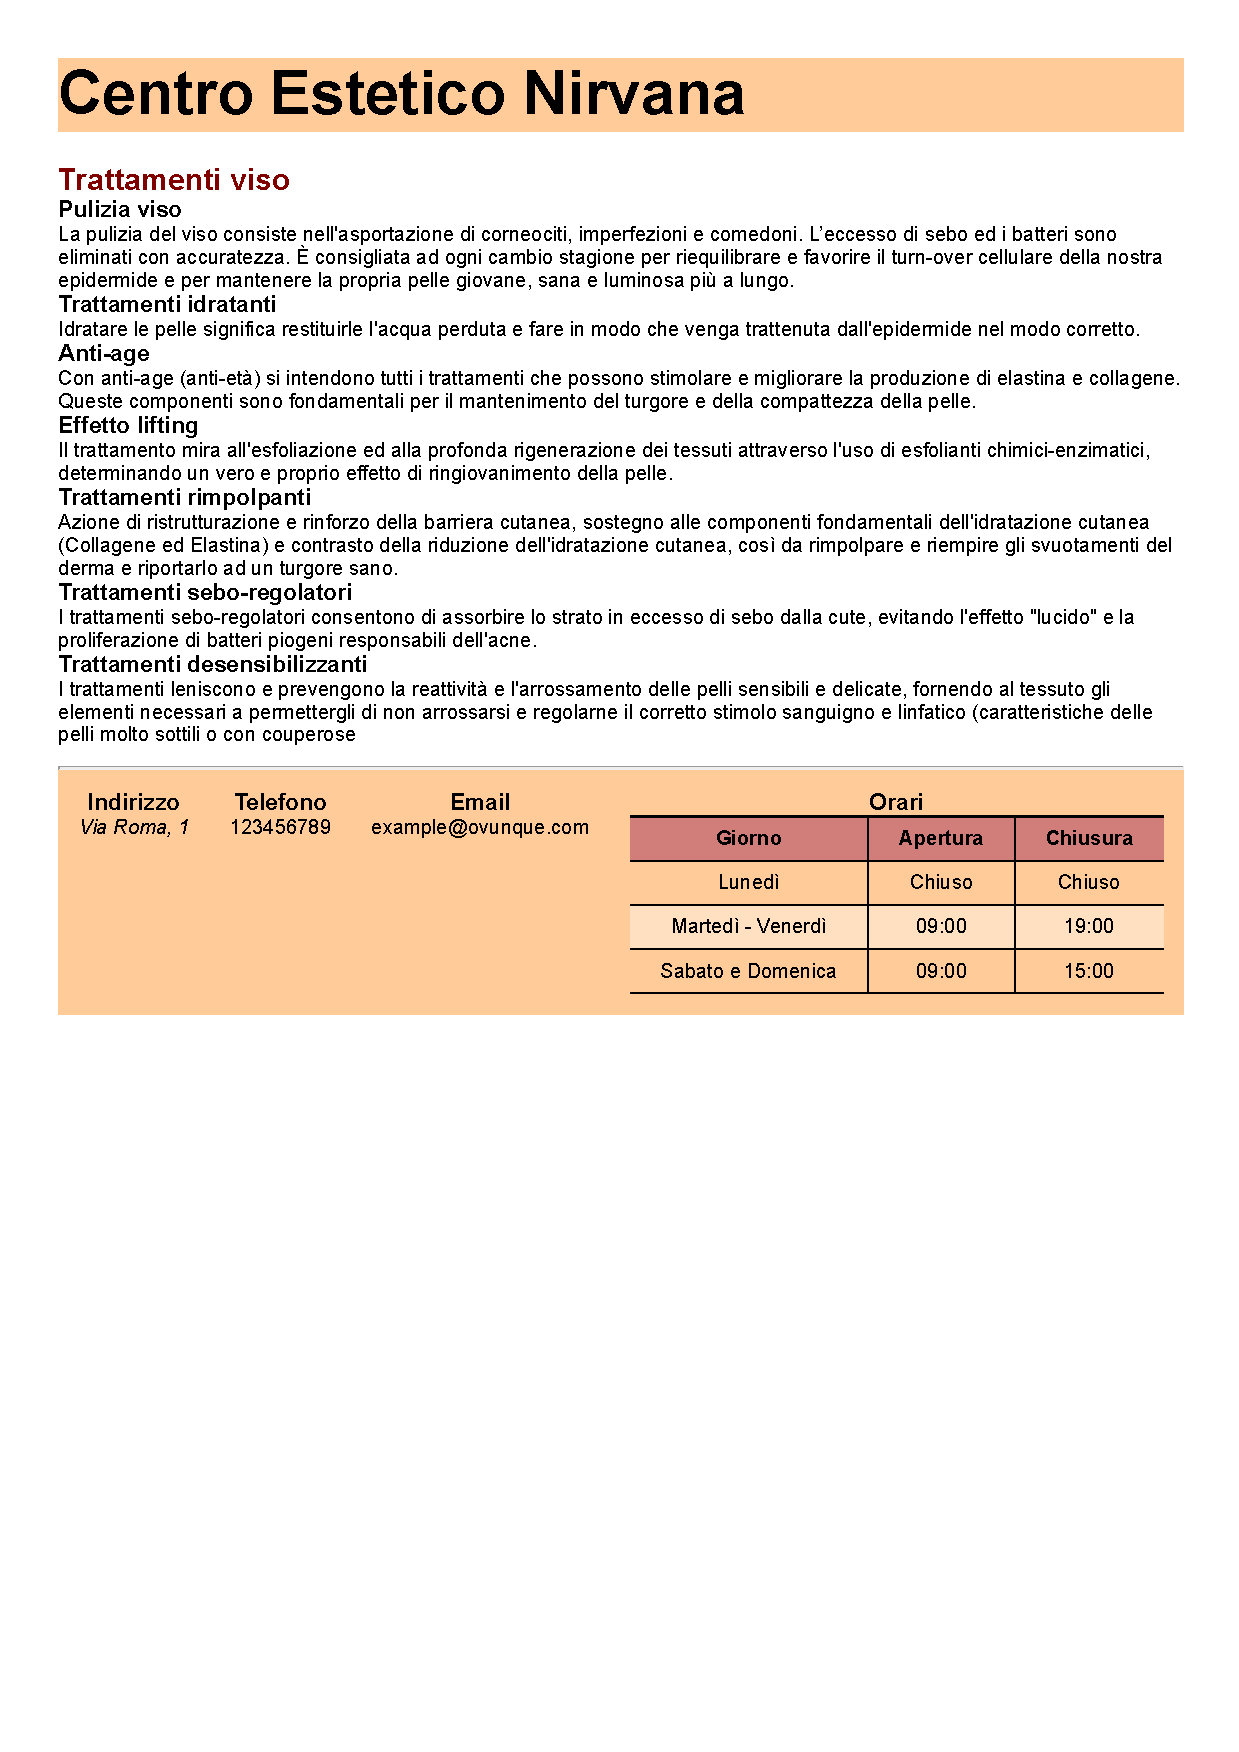
\includegraphics[width=0.5\textwidth]{./graphics/NirvanaTrattamentiViso-w.pdf}}
	\fbox{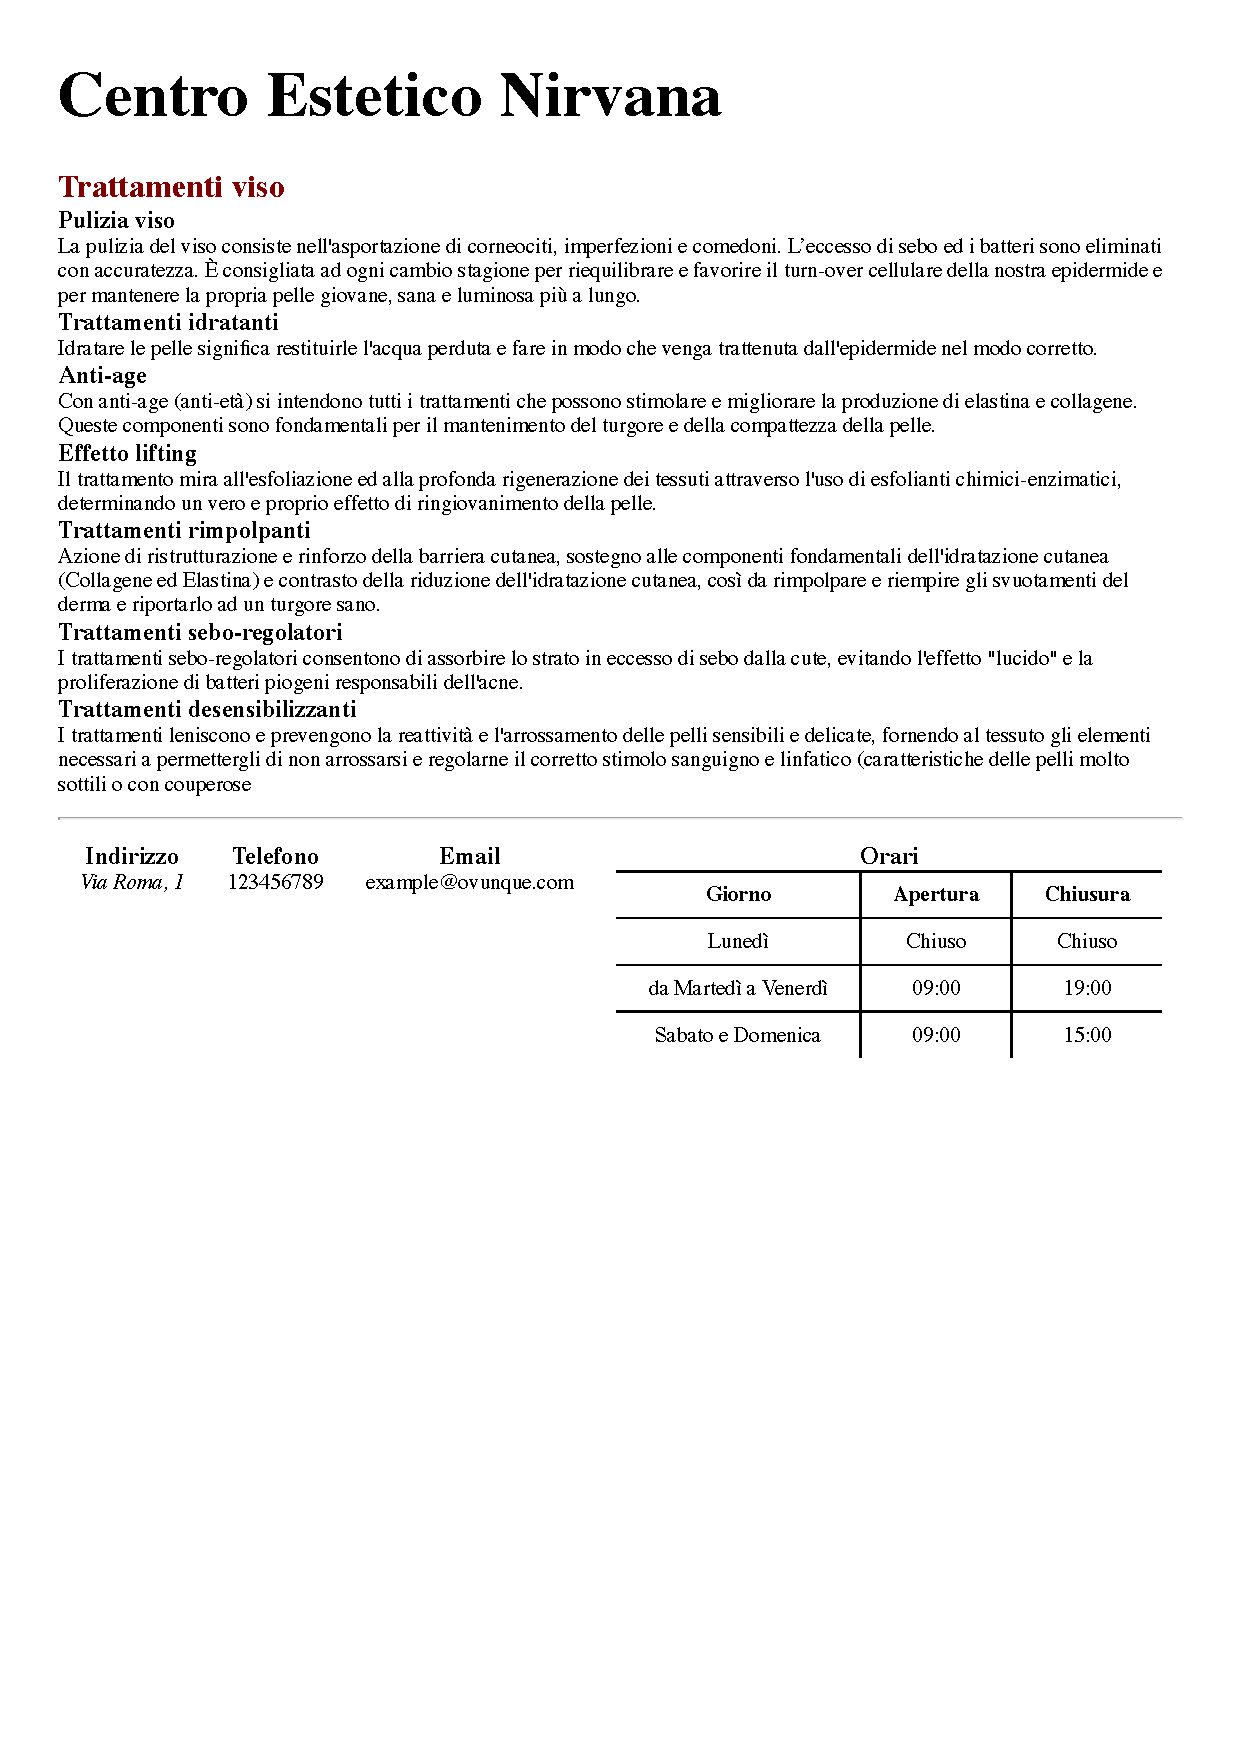
\includegraphics[width=0.5\textwidth]{./graphics/NirvanaTrattamentiViso-wo.pdf}}
%includere l'uso di font con le grazie
%dire dei cambiamenti recenti

%nuova sezione
\section{Implementazione}
\subsection{Linguaggi}		
\subsubsection{HTML e CSS}	%Annalisa e Matteo
\subsubsection{PHP} % Matteo e Nicola
\subsubsection{SQL}	% Nicola
\subsubsection{JavaScript} %Lisien

%nuova sezione
\section{Validazione}

%nuova sezione
\section{Fase di Test}

%nuova sezione
\section{Strumenti}
A supporto dello sviluppatore, é necessario che siano presenti degli strumenti per guidarlo in uno sviluppo efficiente e in un testing accurato.\\
Vengono sottolineate due categorie di strumenti poiché alcuni strumenti utilizzati non sono adatti per una fase di test, ma risultano estremamente utili come aiuto allo sviluppo.
\subsection{Strumenti di sviluppo}
\subsection{Strumenti di test}
\section{Suddivisione del lavoro}
Per garantire una buona suddivisione del carico di lavoro che il progetto ha inevitabilmente richiesto, si é suddiviso il lavoro tra i membri del gruppo in questo modo:
\begin{itemize}
	\item Lisien Skenderi: 
	\begin{itemize}
		\item HTML: Sviluppo delle seguenti pagine: Index, Consulenze, Gestione Prenotazioni - Cliente;
		\item CSS:  elaborazione coordinata del file style.css con particolare attenzione alle sezioni header e breadcrumb
		\item Javascript: Sviluppo delle funzioni per i menú
		\item PHP:
		\item Immagini:
		\item Relazione:
	\end{itemize}
	\item Matteo Cusin:
	\begin{itemize}
		\item HTML: Sviluppo delle seguenti pagine: Trattamenti Viso, Login e Registrazione, Eliminazione prenotazioni;
		\item CSS: creazione e sviluppo di mobile.css, elaborazione coordinata del file style.css con particolare attenzione alle sezioni footer e main
		\item Javascript:
		\item PHP:
		\item Immagini: compressione delle immagini utilizzate ed eliminazione delle immagini non utilizzate
		\item Relazione:
	\end{itemize} ;
	\item Annalisa Egidi:
	\begin{itemize}
		\item HTML: Sviluppo coordinato delle seguenti pagine: 404, areaPersonale, file di trattamenti e index /**/;
		\item CSS: creazione e sviluppo di print.css, elaborazione coordinata del file style.css con particolare attenzione alle sezioni footer e main
		\item Javascript: /**/
		\item PHP: /**/
		\item Immagini: ricerca e modifica coordinata delle immagini, implementazione codice per l'utilizzo delle stesse.
		\item Relazione: /**/
	\end{itemize} ;
	\item Nicola Baesso:
	\begin{itemize}
		\item HTML: Sviluppo delle seguenti pagine: ;
		\item CSS:
		\item Javascript:
		\item PHP: backend dei form di login e registrazione, backend prenotazioni lato amministratore e cliente
		\item Immagini:
		\item Relazione:
	\end{itemize} ;
\end{itemize}

\end{document}
